\subsection{properties of triangles}

\textit{Apply and justify properties of triangles (e.g., the \textbf{Exterior Angle Theorem}, \textbf{concurrence theorems}, \textbf{trigonometric ratios}, \textbf{triangle inequality}, \textbf{Law of Sines}, \textbf{Law of Cosines}, the \textbf{Pythagorean Theorem} and its \textbf{converse})}

\subsubsection{Exterior Angle Theorem}

\begin{figure}[h!]
    \centering
    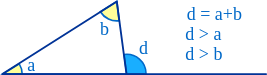
\includegraphics[width=4cm]{./public/images/exterior-angle-theorem}
    \caption[exterior-angle]{exterior angle theorem}
\end{figure}

\vspace{4cm}

\subsubsection{concurrence theorems}

\begin{figure}[h!]
    \centering
    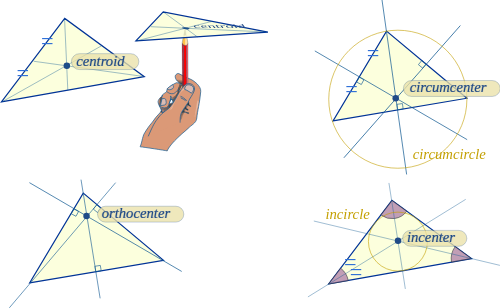
\includegraphics[width=8cm]{./public/images/triangle-centers}
    \caption{triangle centers}
\end{figure}

\paragraph*{centroid} Draw a line (called a "median") from each corner to the midpoint of the opposite side.
Where all three lines intersect is the centroid, which is also the "center of mass":

\begin{figure}[h!]
    \centering
    \begin{subfigure}{2cm}
        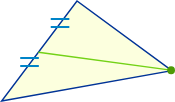
\includegraphics[width=2cm]{./public/images/median}
        \caption{median}
    \end{subfigure}
    \begin{subfigure}{3cm}
        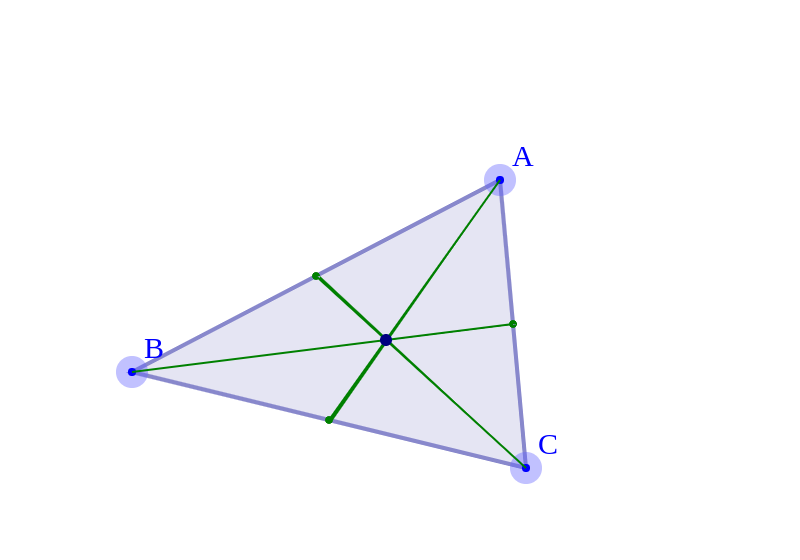
\includegraphics[width=3cm]{./public/images/centroid}
        \caption{centroid}
    \end{subfigure}
    \caption{median $\implies$ centroid}
\end{figure}

\paragraph*{circumcenter} Draw a line (called a "perpendicular bisector") at right angles to the midpoint of each side.Where all three lines intersect is the center of a triangle's "circumcircle", called the "circumcenter":

\begin{figure}[h!]
    \centering
    \begin{subfigure}{3cm}
        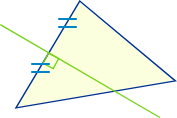
\includegraphics[width=2.5cm]{./public/images/perpendicular-bisector}
        \caption{perpendicular bisector}
    \end{subfigure}
    \begin{subfigure}{3cm}
        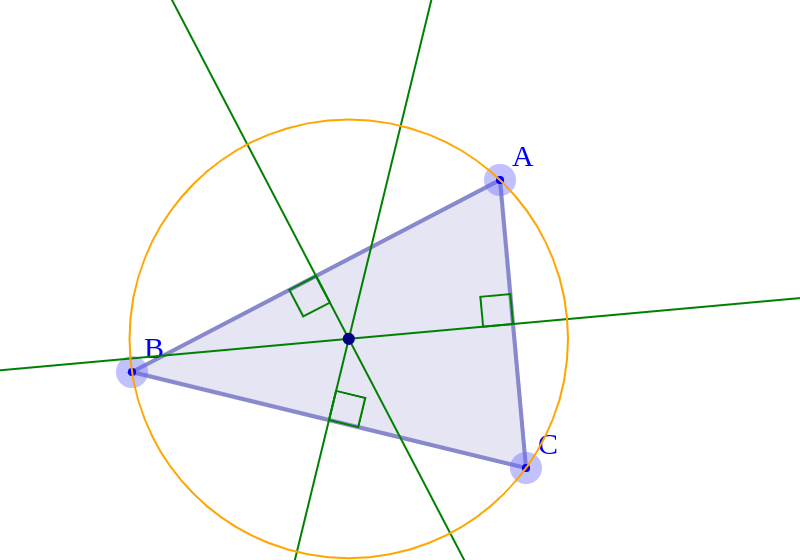
\includegraphics[width=3cm]{./public/images/circumcenter}
        \caption{circumcenter}
    \end{subfigure}
    \caption{perpendicular bisector $\implies$ circumcenter}
\end{figure}


\paragraph*{incenter} Draw a line (called the "angle bisector") from a corner so that it splits the angle in half
Where all three lines intersect is the center of a triangle's "incircle", called the "incenter":

\begin{figure}[h!]
    \centering
    \begin{subfigure}{3cm}
        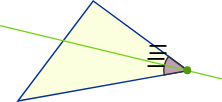
\includegraphics[width=2.5cm]{./public/images/angle-bisector}
        \caption{angle bisector}
    \end{subfigure}
    \begin{subfigure}{3cm}
        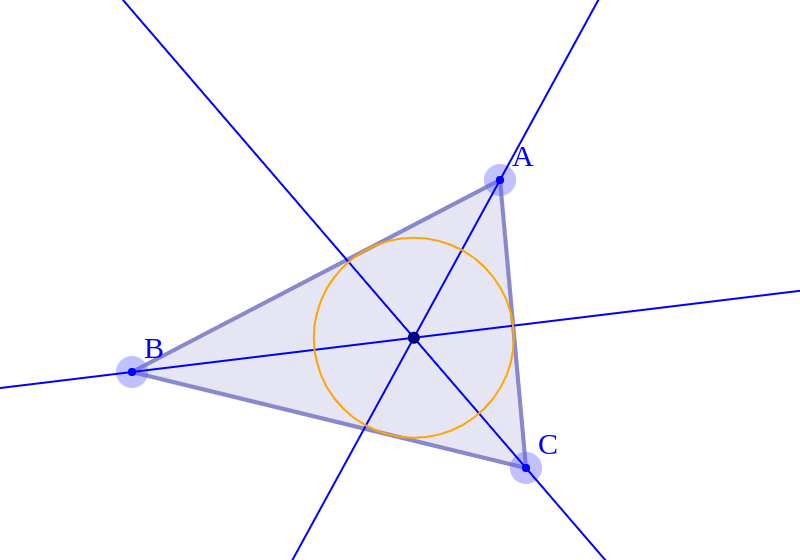
\includegraphics[width=3cm]{./public/images/incenter}
        \caption{incenter}
    \end{subfigure}
    \caption{angle bisector $\implies$ incenter}
\end{figure}
\subsubsection{trigonometric ratios} 

\subsubsection{triangle inequality}

\subsubsection{Law of Sines}

\subsubsection{Law of Cosines}

\subsubsection{Pythagorean Theorem}

\subsubsection{Pythagorean Theorem (converse)}